\subsection{Optimale Anzahl an Samples pro Level}
In diesem Kapitel sei die Anzahl an Level $L\in\mathbb{N}$ mit $L\geq K$, sowie die Fehlertoleranz $\varepsilon\in (0,\infty)$ fest. Hierbei ist $K$ eine Konstante, die wir im Verlauf des Kapitels herleiten werden. Wir wollen herausfinden, wie die Anzahl an Monte Carlo Samples $(n_l)_{l=1}^L$ f"ur jedes Level optimal zu w"ahlen ist. Genauer sind wir an der optimalen L"osung des folgenden Problems interessiert.
\begin{align*}
\min_{(n_1,...,n_L) \in\mathbb{N}^L}\text{cost}\left(\mathcal{M}_L^{\text{MLMC}} ((n_l)_{l=1}^L)\right)=\min_{(n_1,...,n_L) \in\mathbb{N}^L} \ \sum_{l=1}^Ln_l(\text{cost}(add_E)+\text{cost}(D_l))
\end{align*}
mit
\begin{align*}
\|\mathcal{M}_L^{\text{MLMC}} ((n_l)_{l=1}^L)-a\|_{L^p(\Omega;E)}\leq \varepsilon.
\end{align*}
Da uns kein expliziter Ausdruck f"ur $\text{cost}\left(\mathcal{M}_L^{\text{MLMC}} ((n_l)_{l=1}^L)\right)$ und\\ $\|\mathcal{M}_L^{\text{MLMC}} ((n_l)_{l=1}^L)-a\|_{L^p(\Omega;E)}$ vorliegt, verwenden  wir \eqref{c} und die Voraussetzung \ref{v}.
Die Gleichung \eqref{c} besagt, dass
\begin{align*}
\|a-\mathcal{M}_L^{\text{MLMC}}((n_l)_{l=1}^L)\|_{L^p(\Omega;E)}\leq C_1 h^{q_1L}+2C_2 T_p(E)\left(\sum_{l=1}^L \frac{h^{p q_2 l}}{n_l^{p-1}}\right)^{\frac{1}{p}}
\end{align*} gilt.
In diesem Kapitel nehmen wir an, dass beide Summanden gleich viel zu $\varepsilon$ beitragen.
Wir w"ahlen also $L\in\mathbb{N}$ gro"s genug, sodass $C_1h^{q_1L}<\frac{\varepsilon}{2}$ gilt. F"ur $L$ folgt damit:
\begin{align}
C_1h^{q_1L}<&\frac{\varepsilon}{2} \nonumber \\ \nonumber
\Leftrightarrow \log(C_1)+q_1L\log(h)<&\log(\varepsilon)-\log(2)\\
\Leftrightarrow q_1L\log(h)<&\log(\varepsilon)-\log(2)-\log(C_1)\nonumber\\
\Leftrightarrow L>&\frac{\log(\varepsilon)-\log(\frac{2}{C_1})}{q_1\underbrace{\log(h)}_{<0}}=:K. \label{L1}
\end{align}
F"ur unser Problem muss also $L>\frac{\log(\varepsilon)-\log(\frac{1}{\pi\sqrt{3}})}{\log(\frac{1}{2})}$ gelten.
Wir w"ahlen  $L:=\left\lceil \frac{\log(\varepsilon)-\log(\frac{1}{\pi\sqrt{3}})}{\log(\frac{1}{2})} \right\rceil$
und mit der Voraussetzung \ref{v} erhalten wir das vereinfachte Problem
\begin{align}
\min_{(n_1,...,n_L)\in\mathbb{N}^L} \ \sum_{l=1}^L n_lC_3h^{-rl}
\end{align}
mit
\begin{align}
\|a-\mathcal{M}_L^{\text{MLMC}}((n_l)_{l=1}^L)\|_{L^p(\Omega;E)}\leq &C_1 h^{q_1L}+2C_2 T_p(E)\left(\sum_{l=1}^L \frac{h^{p q_2 l}}{n_l^{p-1}}\right)^{\frac{1}{p}}\leq\varepsilon\\
\Leftrightarrow
\sum_{l=1}^L \frac{h^{pq_2l}}{n_l^{p-1}}\leq& (2C_2T_p(E))^{-p}(\varepsilon-C_1h^{q_1L})^p.
\end{align}
F"ur das folgende Lemma ben"otigt man im Beweis die H"olderungleichung f"ur die Folgenr"aume. 
\begin{sz}[H"olderungleichung]
Es sei $1<p<q<\infty$ und $\frac{1}{p}+\frac{1}{q}=1$ so gilt f"ur $\textbf{x}\in \ell^p$ und $\textbf{y}\in \ell^q$, dass $\{x_ny_n\}_{n\in\mathbb{N}}\in\ell^1$ und
\begin{align*}
\|\{x_ny_n\}\|_{\ell^1}\leq\|\textbf{x}\|_{\ell^p}\cdot\|\textbf{y}\|_{\ell^q} \ \ \text{mit} \ \|\textbf{x}\|_{\ell^p}=\left(\sum_{n=1}^\infty |x_n|^p\right)^{\frac{1}{p}}.
\end{align*}
\end{sz}
\begin{proof}
Hierbei orientiere ich mich an \cite{Holder}.
F"ur den Beweis ben"otigen wir folgenden Hilfssatz
\begin{sz}
F"ur $p,q \in [0,\infty)$ mit
\begin{equation*}
\frac{1}{p}+\frac{1}{q}=1
\end{equation*} und $a,b\geq 0$ gilt
\begin{equation*}
ab\leq \frac{a^p}{p}+\frac{b^q}{q}.
\end{equation*}
\end{sz}
\begin{proof}
Wir betrachten f"ur $x\in(0,\infty)$ die Funktion
\begin{eqnarray*}
g(x)=\frac{x^p}{p}+\frac{1}{qx^q}.
\end{eqnarray*}
Dann ist $g'(x)=x^{p-1}-x^{-q-1}$. Damit ist die Funktion monoton fallend auf dem Intervall $(0,1)$ und  monoton steigend f"ur $(1,\infty)$. Die einzige Nullstelle der Ableitung liegt bei $x=1$ und liefert den Funktionswert $g(1)=\frac{1}{p}+\frac{1}{q}=1$. Damit ist $g\geq 1$. Setzen wir nun $x=a^{\frac{1}{q}}\cdot b^{-\frac{1}{p}}$ erhalten wir
\begin{align*}
1\leq g(x) = \frac{a^{\frac{p}{q}}}{pb}+\frac{b^{\frac{q}{p}}}{qa}.
\end{align*}
Nach Multiplikation mit $ab$ gilt
\begin{align*}
ab\leq\frac{a^{1+\frac{p}{q}}}{p}+\frac{b^{1+\frac{q}{p}}}{q}.
\end{align*}
Nun kann man die urspr"ungliche Gleichung $\frac{1}{p}+\frac{1}{q}=1$ umschreiben zu $p+q=pq$ oder $1+\frac{p}{q}=p,$ bzw. $1+\frac{q}{p}=p$.\\
Dies ergibt die gew"unschte Formel.
\end{proof}
Wir setzen
\begin{align*}
s_n=\frac{|x_n|^p}{\|\textbf{x}\|_{\ell^p}^p}; t_n=\frac{|y_n|^p}{\|\textbf{y}\|_{\ell^q}^q}.
\end{align*}
Dann gilt mit obigen Hilfssatz
\begin{align*}
|s_n|^{\frac{1}{p}}|t_n|^{\frac{1}{q}}\leq \frac{1}{p}|s_n|+\frac{1}{q}|t_n|.
\end{align*}
Damit ist
\begin{align*}
\frac{1}{\|\textbf{x}\|_{\ell^p}\|\textbf{y}\|_{\ell^q}}\sum_{j=1}^n|x_jy_j|\leq \frac{1}{p\|\textbf{x}\|_{\ell^p}^p}\sum_{j=1}^n|x_j|^p+\frac{1}{q\|\textbf{y}\|_{\ell^q}^q}\sum_{j=1}^n|y_j|^q\leq\frac{1}{p}+\frac{1}{q}=1.
\end{align*}
F"ur $n\rightarrow \infty$ wird die rechte Ungleichung zur Gleichung und es folgt
\begin{align*}
\|\{x_ny_n\}\|_{\ell^1}\leq\|\textbf{x}\|_{\ell^p}\cdot\|\textbf{y}\|_{\ell^q} 
\end{align*}
\end{proof}
\begin{lem}\label{opt}
Sei $\delta\in(0,\infty),L\in\mathbb{N}$, und sei $(b_l)_{l=1}^L,(c_l)_{l=1}^L\subset\mathbb{R}$ zwei gegebene Folgen von positiven reellen Zahlen. Die eindeutige L"osung des Minimierungsproblems
\begin{align*}
\min_{(a_1,...,a_L)\in\mathbb{R}^L} \ \sum_{l=1}^L c_la_l
\end{align*}
mit
\begin{align*}
\sum_{l=1}^L \frac{b_l^p}{a_l^{p-1}}=\delta^p, \ \ a_l>0, \forall\  l=1,...,L
\end{align*}
ist gegeben durch
\begin{align*}
a_l^*:=\delta^{-\frac{p}{p-1}} b_l c_l^{-\frac{1}{p}}\left(\sum_{k=1}^L c_k^{\frac{p-1}{p}}b_k\right)^{\frac{1}{p-1}}, \ \ l=1,...,L.
\end{align*}
\end{lem}
\begin{proof}
Es ist einfach nachzuweisen, dass $(a_1^*,...,a_L^*)\in\mathbb{R}^L$ eine geeignete L"osung ist. Wir definieren f"ur $(a_1,...,a_L)\in\mathbb{R}^L$
\begin{align*}
V(a_1,...,a_L):=\sum_{l=1}^L c_la_l.
\end{align*}
Dann folgt:
\begin{align*}
V(a_1^*,...,a_L^*)=\delta^{-\frac{p}{p-1}}\left(\sum_{k=1}^L c_k^{\frac{p-1}{p}}b_k\right)^{\frac{1}{p-1}}\left(\sum_{l=1}^L c_l^{\frac{p-1}{p}}b_l\right)=\delta^{-\frac{p}{p-1}}\left(\sum_{l=1}^L c_l^{\frac{p-1}{p}}b_l\right)^{\frac{p}{p-1}}.
\end{align*}
Es ist
\begin{align*}
\delta^{-\frac{p}{p-1}}\left(\sum_{l=1}^L c_l^{\frac{p-1}{p}}b_l\right)^{\frac{p}{p-1}}=\delta^{-\frac{p}{p-1}}\left(\sum_{l=1}^L(c_la_l)^{\frac{p-1}{p}}\frac{b_l}{a_l^{\frac{p-1}{p}}}\right)^{\frac{p}{p-1}}.
\end{align*} 
Die H"olderungleichung mit den Exponenten $p'=\frac{p}{p-1}$ und $q'=p$ liefert f"ur den Ausdruck in den Klammern f"ur  $(a_1,...,a_L)\in\mathbb{R}^L$
\begin{align}
\sum_{l=1}^L(c_la_l)^{\frac{p-1}{p}}\frac{b_l}{a_l^{\frac{p-1}{p}}}\leq& \left(\sum_{l=1}^L((c_la_l)^{\frac{p-1}{p}})^{\frac{p}{p-1}})\right)^{\frac{p-1}{p}}\cdot \left(\sum_{l=1}^L\left(\frac{b_l}{a_l^{\frac{p-1}{p}}}\right)^p\right)^{\frac{1}{p}}\\
=&\left(\sum_{l=1}^L c_la_l\right)^{\frac{p-1}{p}}\cdot \left(\sum_{l=1}^L\left(\frac{b_l^p}{a_l^{p-1}}\right)\right)^{\frac{1}{p}}.
\end{align}
Dadurch erhalten wir insgesamt
\begin{align*}
\delta^{-\frac{p}{p-1}}\left(\sum_{l=1}^L(c_la_l)^{\frac{p-1}{p}}\frac{b_l}{a_l^{\frac{p-1}{p}}}\right)^{\frac{p}{p-1}}
\leq& \delta^{-\frac{p}{p-1}}\left(\left(\sum_{l=1}^L c_la_l\right)^{\frac{p-1}{p}}\cdot \left(\sum_{l=1}^L\left(\frac{b_l^p}{a_l^{p-1}}\right)\right)^{\frac{1}{p}}\right)^{\frac{p}{p-1}}\\
=&\delta^{-\frac{p}{p-1}}\sum_{l=1}^L(c_la_l)\left(\underbrace{\sum_{l=1}^L\frac{b_l^p}{a_l^{p-1}}}_{=\delta^p}\right)^{\frac{1}{p-1}}=\sum_{l=1}^L c_la_l=V(a_1,...,a_L).
\end{align*}
Dies zeigt, dass 
\begin{align*}
V(a_1^*,...,a_L^*)\leq V(a_1,...,a_L)
\end{align*}
f"ur $(a_1,...,a_L)\in\mathbb{R}^L$ gilt. Die Eindeutigkeit folgt aus der H"olderungleichung in $(7)$.
\end{proof}
 Wir wenden nun dieses Lemma auf unser Problem in $(6)-(8)$ an. Daf"ur setzen wir
 \begin{align}\label{delta}
 \delta:=\frac{\varepsilon-C_1h^{q_1L}}{2C_2T_p(E)},\ \ b_l:=h^{q_2l},\ \ c_l:=C_3h^{-rl}
 \end{align} f"ur $l=1,...,L$.\\
 Als L"osung erhalten wir dann
 \begin{align*}
 a_l^*=\delta^{-\frac{p}{p-1}}b_lc_l^{-\frac{1}{p}}\left(\sum_{k=1}^L c_k^{\frac{p-1}{p}}b_k\right)^{\frac{1}{p-1}}.
 \end{align*}
 Die $a_l^*$ sind jedoch nicht unbedingt ganzzahlig und wir haben ein ganzzahliges Optimierungsproblem zu l"osen.
 Eine M"oglichkeit w"are $n_l^*$ folgenderma"sen zu w"ahlen:
 \begin{align}\label{n}
n_l^*:= \lceil a_l^* \rceil=\Big\lceil  \delta^{-\frac{p}{p-1}}b_lc_l^{-\frac{1}{p}}\left(\sum_{k=1}^L c_k^{\frac{p-1}{p}}b_k\right)^{\frac{1}{p-1}}\Big\rceil \in \mathbb{N}, \ \ l=1,...,L. 
 \end{align}
Dieses Ergebnis liegt nahe am Optimum. Wegen der Nebenbedingung ist nur Aufrunden eine Option, da die $n_l$ im Nenner stehen. Ein Abrunden w"urde die Summe vergr"o"sern und damit die Nebenbedingung verletzten.\\
Es ist zu erkennen, dass $(n_l^*)_{l\in\mathbb{N}}$ nicht von der Konstante $C_3$ abh"angt.
Denn diese Konstante $C_3$ steckt in jedem Summanden und kann deshalb ausgeklammert werden. Deshalb erhalten wir
\begin{align*}
n_l^*:= \lceil a_l^* \rceil=\Big\lceil  \delta^{-\frac{p}{p-1}}b_l (C_3)^{-\frac{1}{p}}( h^{-rl})^{-\frac{1}{p}}(C_3^{\frac{p-1}{p(p-1)}})\left(\sum_{k=1}^L (h^{-rl})^{\frac{p-1}{p}}b_k\right)^{\frac{1}{p-1}}\Big\rceil \in \mathbb{N}, \ \ l=1,...,L. 
\end{align*}
D.h der Faktor $C_3$ k"urzt sich raus. Trotzdem ist f"ur die Implementierung des MLMC-Algorithmus mit $(n_l^*)_{l\in\mathbb{N}}$ die genaue Kenntnis der Konstanten $C_1,C_2,T_p(E),h$, der Raten $q_1,q_2$ und $r$ notwendig.
\newpage
Das Lemma liefert uns folgende Ergebnisse f"ur die optimale Sampleanzahl:

\begin{enumerate}
\item[-]$\varepsilon=10^{-1}$: F"ur diese Fehlerschranke gilt L=2.\\[0,3cm]

\begin{tabular}{|c|c|c|}
Sampleanzahl &Level 1 & Level 2 \\
 \hline
&2629 & 930 \\
\end{tabular}\\[0,3cm]
Die Ergebnisse von $a(\lambda)$ sind\\[0,3cm]

\begin{tabular}{|c|c|c|c|c|c|}
$\lambda$ & $0.1$&$0.3$&$0.5$&$0.7$&$1$  \\
 \hline
$a(\lambda)$& $0.0619$  &  $0.2512$  &  $0.3286$&    $0.5048$  &  $0.6493$\\
\end{tabular}\\

\begin{figure}[h]
\centering
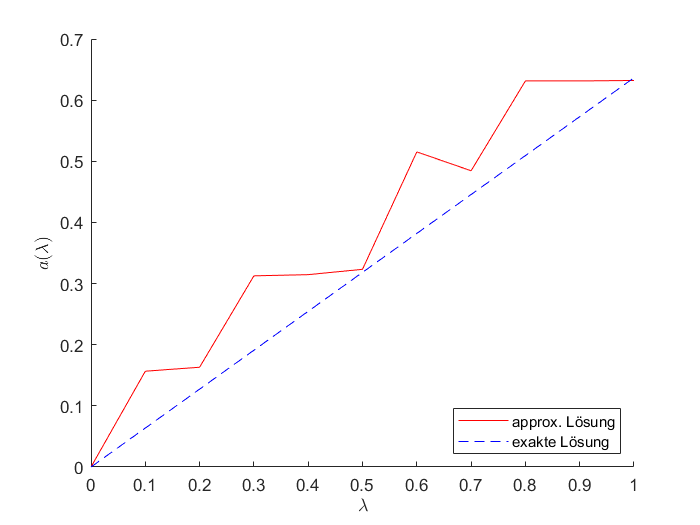
\includegraphics[width=13cm]{epsilon-1.png}
\end{figure}
\newpage

\item[-]$\varepsilon=10^{-2}$: F"ur diese Fehlerschranke gilt L=6.\\[0,3cm]

\begin{tabular}{|c|c|c|c|c|c|c|}
Sampleanzahl &Level 1 & Level 2&Level 3&Level 4&Level 5& Level 6 \\
 \hline
& 16703    &    5906    &    2088     &    739    &     261 &  93\\
\end{tabular}\\[0,3cm]

Es ist zu erkennen, wie viel mehr Samples und Level man ben"otigt um den Fehler um eine Nachkommastelle zu verbessern.
Die Ergebnisse von $a(\lambda)$ sind\\[0,3cm]

\begin{tabular}{|c|c|c|c|c|c|}

$\lambda$ & $0.1$&$0.3$&$0.5$&$0.7$&$1$  \\
 \hline
$a(\lambda)$&  0.0584  &  0.1947 &  0.3204 &   0.4537 &   0.6414\\
\end{tabular}\\

\begin{figure}[h]
\centering
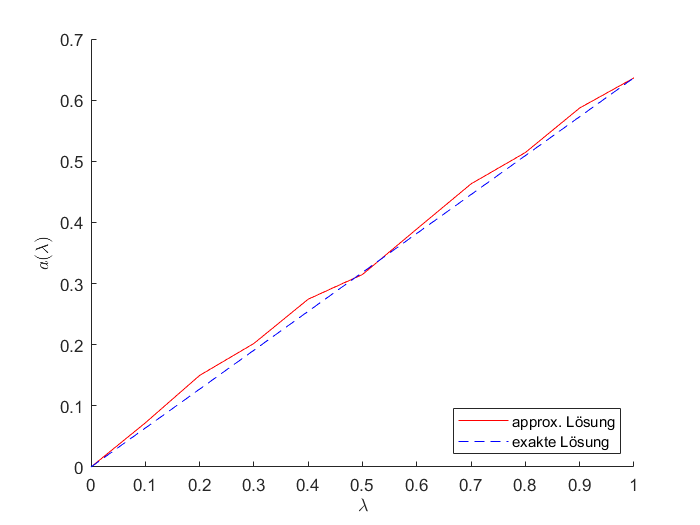
\includegraphics[width=13cm]{epsilon-2.png}
\end{figure}

\newpage

\item[-]$\varepsilon=10^{-3}$:
F"ur diese Fehlerschranke gilt L=9.\\[0,3cm]

\begin{tabular}{|c|c|c|c|c|c|c|}
Sampleanzahl &Level 1 & Level 2&Level 3&Level 4&Level 5& Level 6\\
 \hline
& 4154140   &  1468711  &    519268  &    183589     &  64909 & 22949 \\ 
\end{tabular}\\[0,3cm]

\begin{tabular}{|c|c|c|}
 Level 7 & Level 8 & Level 9\\
 \hline
  8114   &     2869&   1015\\
\end{tabular}\\[0,3cm]
Die Ergebnisse von $a(\lambda)$ sind\\[0,3cm]
\begin{tabular}{|c|c|c|c|c|c|}

$\lambda$ & $0.1$&$0.3$&$0.5$&$0.7$&$1$  \\
 \hline
$a(\lambda)$&  0.0646  &  0.1911  &  0.3183   & 0.4430 &   0.6364\\
\end{tabular}
\begin{figure}[h]
\centering
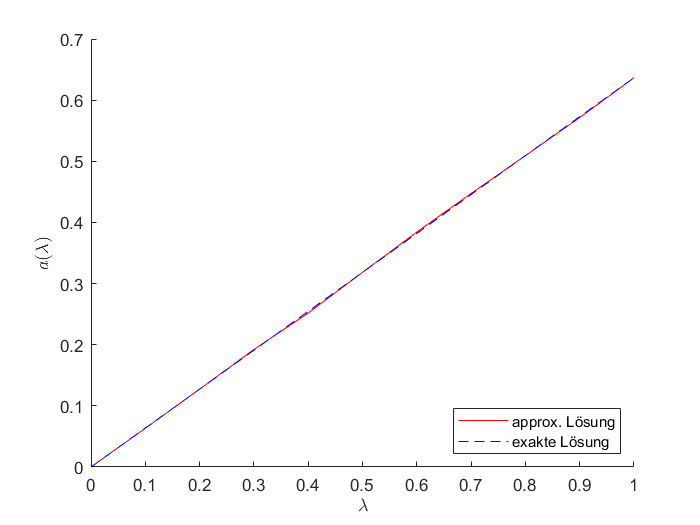
\includegraphics[width=12cm]{epsilon-3.png}
\end{figure}

\item[-]$\varepsilon=10^{-4}$: \\
Ab diesem Fehler war es mir nicht mehr m"oglich mit Matlab die Ergebnisse f"ur $a(\lambda)$ zu bestimmen, da die optimale Sampleanzahl zu gro"s ist.\\
F"ur diese Fehlerschranke gilt L=12.\\[0,3cm]
\begin{tabular}{|c|c|c|c|c|c|c|}
Sampleanzahl &Level 1 & Level 2&Level 3&Level 4&Level 5& Level 6\\
 \hline
$1.0e+09 *$& 3.2314  &  1.1425 &   0.4039   & 0.1428  &  0.0505   & 0.0179  
\end{tabular}\\[0,3cm]
\begin{tabular}{|c|c|c|c|c|c|c|}
 & Level 7 & Level 8 & Level 9& Level 10 &Level 11& Level 12\\
 \hline
$1.0e+09 *$  &  0.0063  &  0.0022 &   0.0008 &  0.0003  &  0.0001 &   0.0000
\end{tabular}\\[0,3cm]

\end{enumerate}

 

 
